\documentclass[conference]{IEEEtran}
\usepackage[utf8]{inputenc}
\usepackage{graphicx}
\usepackage{listings}
\usepackage{url}

%opening
\title{A Dynamic End-to-End Security for Coordinating Multiple Protections within a Linux Desktop}

\author{\IEEEauthorblockN{Jeremy Briffaut}
\IEEEauthorblockA{ENSI de Bourges - LIFO\\
88 Boulevard Lahitolle\\
18020 BOURGES CEDEX, FRANCE\\
Email: jeremy.briffaut@ensi-bourges.fr}
\and
\IEEEauthorblockN{Martin Peres}
\IEEEauthorblockA{ENSI de Bourges\\
Email: martin.peres@ensi-bourges.fr\\
Contact: http://mupuf.org/contact/}
\and
\IEEEauthorblockN{Christian Toinard}
\IEEEauthorblockA{ENSI de Bourges - LIFO\\
88 Boulevard Lahitolle\\
18020 BOURGES CEDEX, FRANCE\\
Email: christian.toinard@ensi-bourges.fr}}

\begin{document}

\maketitle

\begin{IEEEkeywords}
	end-to-end security, multi-domains, protection mechanisms, coordination, Linux.
\end{IEEEkeywords}

\begin{abstract}
	Currently,  application protection models are mostly static and independant. 
It means that the applications cannot handle multiple domains to manage accordingly the permissions for a given user request.
	Managing multiple domains is becoming a more and more common issue as desktop applications are growing in complexity to provide better-designed user interfaces.
	Today, protection systems are almost everywhere. Multiple systems of protection are available from the Linux kernel such as SELinux or PIGA-Protect to get a Mandatory Protection. Those systems provide a per-syscall validation process. Network protections are also available such as the IPtables firewalling mechanism. Protections for languages or frameworks also exist such as for Java or .NET. But, solutions are missing for coordinating the various mechanisms that protect different levels of the global information system. The purpose is to reuse and coordinate efficiently those different levels of protection in order to provide a end-to-end protection that manages dynamically multiple domains. Thus, the same host can support multiple domains for the user requests while providing a transparent end-to-end security that protects against complex scenarios of attack. This paper describes an attempt to deliver such a system for controlling efficiently the user requests.
\end{abstract}

\section{Introduction}


		Nowadays, protection models ~\cite{LAHMADI:2009:INRIA-00404853:1} ~\cite{1542244} ~\cite{4223222} ~\cite{firefox_ccr_2009}  are mostly based on several security components like firewalls, discretionary access control, mandatory access control or security plugins. Each of them has its own protection policy. ~\cite{BBLT09} considers dynamic MAC policies whereas ~\cite{GM} and ~\cite{ 10.1109/CSFW.2002.1021825} deal with how to manage multi-level models or information flows at a single level of an information system. ~\cite{TELECOM_BRETAGNE-7660} deals with the deployment of security policies accross an organization.

		However, all those protection mechanisms are configured separatly, there are no systems to ''glue'' them all together consistently in order to adjust the various protection policies according to the activities. For example, it is almost impossible to coordinate those protection policies in order to confine an activity such as a bank transfer or the payment of taxes carried out from an ordinary Web Browser. This means, the user have the same amount of rights when watching a movie or when he is paying his/her taxes on the Internet.

		For instance, a firewall is agnostic to a browser events. This means it cannot open and close ports according to the URL a user is visiting.
		Also, a SELinux-based MAC policy is not changing to fit the application's current needs. A MAC policy is designed to fit every single need the application could have.

		This is a direct violation of the principle of least privilege.

		To overcome this limitation, the computer needs several sets of permissions (domain) according to the different activities the user may have on it.

		A domain is defined by the minimum amount of permissions to allow a user to carry out an activity. There should be as many domains as there are activities.

		For instance, when a user wants to buy something on the Internet, he will automatically transit to the domain \texttt{eshopping}. 
		In this domain, he/she will be able to browse the website, read mails from this website, read his/her bank account number and send mails to this website.

		A domain should be configured in order to apply the principle of least privilege. 
		The purpose is to offer a end-to-end  protection going from the lower layers of the kernel to the user-interface through the network.

		A domain transition occurs when the user changes his/her activity. The change of activity can be detected easily by watching the mail or the URL the user is visiting. 
		For instance, if the user leaves \url{http://www.ebay.com/} to go to \url{http://www.cnn.com/}, we can know for sure he/she is not shopping anymore. 
		Thus, we can switch from the domain \texttt{eshopping} to the domain \texttt{web}.

		A dynamic domain-based end-to-end protection can be represented as a finite-state machine where states would represent domains and where transitions would be possible application requests. Our architecture captures those requests in order to install dynamically the required protection policies for the various levels of the information system.

\section{Architecture}
		In order to achieve an application-level protection, one needs a system which receives application transition requests and  match them with the finite-state machine.
		If a request matches a transition rule, then the system should change its domain to comply with the new domain. 
		Otherwise, the application which had sent the request shouldn't perform the concerned operation. 

		This system should be composed of a privileged daemon, capable of switching from a domain to another, and of a
		mean of communication between the daemon and the applications which require a dynamic protection model.

		It is a form of mandatory access control which can also grant privileges.

		\subsubsection{Userspace communication}
			\paragraph{Registration} To interact with the daemon, an application first has to register itself. The registration request is composed of a name (must be unique) and of a PID. 
			The daemon checks the PID of the application and retrieves the path of the binary associated on the file system.
			Given this, the daemon looks into its configuration file and tells whether the application is known and allowed to register. If the application's request is denied,
			it will not be allowed for the application to communicate with the daemon.

			\begin{figure}[h!]
				\centering
				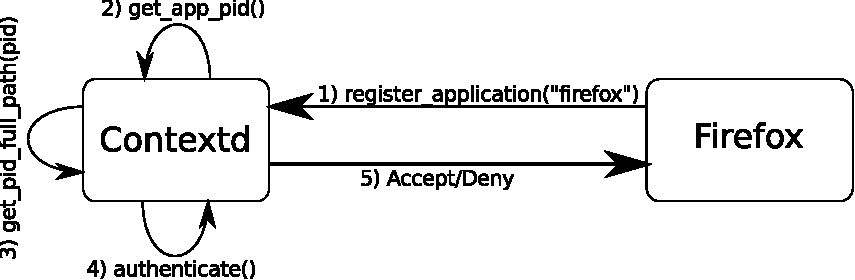
\includegraphics[scale=0.6]{app_authentication.pdf}
				\caption{Example of a registration process between Firefox and Contextd}
				\label{app_registration}
			\end{figure}

			\paragraph{Context change} 
			Whenever an application wants to switch to a new context of execution - ie. to do something else - this application should do a synchronous IPC request to the daemon.

			The request is made of the name of the process, its PID (accessed using the IPC system) and application-defined relevant variables. 
			For instance, a web-browser willing to reach \url{http://www.google.com} would send a request with these variables:
			{\it protocol=http; host=www.google.com; port=80; path=/}.

			The request will then be matched to the finite-state machine by the daemon and will either be accepted or rejected. When a request is rejected,
			the application mustn't change its internal context or should go to a trash context that could explain the user why the action
			he/she started failed.

			\begin{figure}[h!]
				\centering
				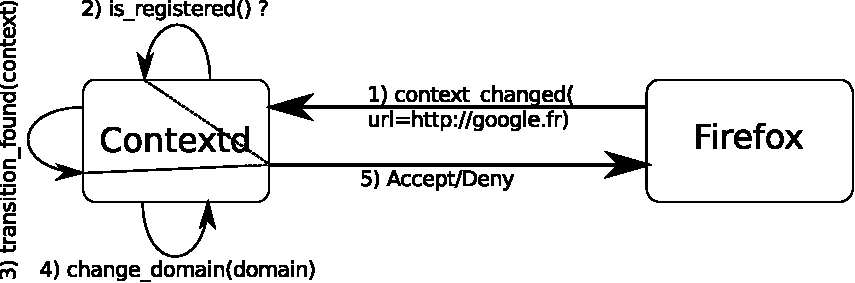
\includegraphics[scale=0.6]{app_contextchanged.pdf}
				\caption{Example of a request of Firefox to visit google.com}
				\label{app_contextchanged}
			\end{figure}

			\paragraph{Integration} 
			The daemon may also force applications to change their inner context. Whenever the daemon switch from one domain to another, it broadcasts
			the name of the domain to registered applications. Applications should then test if their current context is compatible with the daemon's domain 
			and either go to a trash context or keep doing the same thing.

			For instance, let's say Firefox is browsing \url{http://www.ebay.com} while the system is in the domain \texttt{eshopping}. Firefox now receives a message from the daemon
			telling a domain switch has occured from the domain \texttt{eshopping} to the domain \texttt{web}. Firefox now asks the daemon whether 
			the \url{http://www.ebay.com} is acceptable in the \texttt{web} domain. The daemon answers it is not, Firefox has to shut down this page and show a message
			telling the user the webpage has been hidden because it was infringing the current domain's rules. 

			To achieve such a behaviour, applications need some modifications. These can be achieved either by using plugins or 
			by directly modifying the source code of the application. The latter is of course the most secured but plugins don't really hurt the security
			as long as they are mandatory for the application to execute and as long as they are owned by a privileged user(read-only).

		\subsubsection{Contextd: The privileged daemon}
			Its goal is to process the incoming application's request, apply them to the finite-state machine and decide what to do.
			If it is an accepted application context - ie matches a transition in the finite-state machine - it changes the domain according to the matched transition.
			Either way, the application which sent the request is warned whether its transition is allowed or not.

			It is important that the protection model is changed \emph{before} returning to the application. Otherwise, the application may not
			be able to access resources needed by its new domain.

			The domain switching is made by changing the parameters of several security components, may they be firewalls, mandatory access control systems or logging systems.
			The daemon is statically-linked-plugin based and is designed around a notification API to ease the addition of new security components.

			Contextd should have one plugin per security component. These plugins are notified (of domain changes, errors, debug messages and so on)
			using the notification API. Plugins may also need a configuration file, this will be their responsability to handle it separately.


\section{Implementation}

	\subsection{Language}
		Most of the communication languages used in user-space by Contextd are associated with configuration files or messages using XML-based structures.
		XML's tree-based structure allows a great disctinction between application-data and contextd-data which should avoid any problems of injection.

		Also, XML parsers are common nowadays and programmers are used to it.
		
		The main configuration file can be found at /etc/context.d/transitions.xml.

		\subsubsection{Creating domains}
			Domains are represented by a name, a display name and an icon. The display name and the icon are meant for the user interface.

			Converted to the XML syntax, this gives:
			\begin{verbatim}
				<domain name="mail" display_name="E-Mail" 
					icon="/usr/share/icons/evolution.png"/>
				<domain name="taxes" display_name="Taxes" 
					icon="/usr/share/icons/money_coin.png"/>
			\end{verbatim}

		\subsubsection{Applications authentification}
			To allow an application to send data to the daemon, contextd first needs to authenticate it. Here is the syntax to do so:
			\begin{verbatim}
				<program name="firefox" 
				display_name="Firefox" icon="" 
				full_path="/usr/bin/firefox"/>
			\end{verbatim}

			\paragraph*{full\_path} is the path of the executable to be considered as being \texttt{name}. 
			In this example, the only authorized executable to be called firefox will be /usr/bin/firefox.

		\subsubsection{Adding transitions}
			The transition defination is splitted in two parts. The transition's attributes and the application-defined variables that will
			start the transition.

			The transition attributes are relative to the state machine (transit\_from, transit\_to), 
			the application that can initiate the transition (app\_name) and to the user interface (prompt and notify).

			The application-defined variables are the condition to make the transition effective. They are matched using regular expressions.
			The names of these variables try to be as normalized as possible but you can define your own variables if you need it.

			\begin{verbatim}
				<rule app_name="firefox" 
				transit_from="mail" transit_to="taxes" 
				prompt="false" notify="false">
				     <host>www\.impots\.gouv\.fr</host>
				     <path>.*</path>
				     <protocol>(http|https)</protocol>
				</rule>
			\end{verbatim}

			This transition rule's definition should be read this way:
			``if firefox asks to visit the url http(s)://www.impots.gouv.fr/.* and if the system is in the mail domain, then, 
			the system will transit to the taxes domain.''

			\paragraph*{transit\_form} a regular expression which should match the current domain name.

			\paragraph*{transit\_to} the transition destination. This domain should be declared higher in the configuration file.

			\paragraph*{prompt} should be set to true if you want the user to be prompt to accept or deny the transition.
			This behaviour is close to Microsoft's UAC.

			\paragraph*{notify} attributes defines whether the user should be warned of this transition or if it should be a silent one.

			To be matched, this rules needs firefox to send at least the variables \texttt{host}=``www.impots.gouv.fr'', \texttt{path}=``.*'' and \texttt{protocol}=``(http|https)``.
			This means, if firefox wants to visit \url{http://www.impots.gouv.fr/index.php} and the system in currently in the domain \texttt{mail}, 
			then we will transit to the domain \texttt{taxes}.

	\subsection{Interaction between the security components and the applications}
		\subsubsection{Security components}
			\paragraph*{IPTables} is the most common firewall on Linux desktops and servers. It is available for the 2.4 and the 2.6 Linux kernels and has been around for a while.
			This is a simple and well-known stateful firewall. It can be administrated using a simple command line utility called iptables.

			\paragraph*{SELinux} allow to define a fine-grained MAC policy down to the syscall. By using it, it is possible to deny a direct access to a particular ressource  but you could fool it by using an intermediate operation or process. The administration can be done using modules. Modules can be hot-pluggled and unplugged using a simple command line.

			\paragraph*{PIGA} ~\cite{BBLT09} sits on-top of SELinux and can guarantee a large range of confidentiality and integrity properties.
			In contrast with SELinux, SELinux+PIGA can guarantee an application will never have access to a ressource, even with a lot of intermediate operations and processes.
			Some of the PIGA policies can be updated on the fly.

			\paragraph*{Syslog-NG} is a common logging system on Linux. It allows to log application data, to sort them by urgency and category and to write them to different files.

		\subsubsection{User applications}
			\paragraph*{Firefox} is the second-most used web browser nowadays. It features a powerful and flexible plugin system. 
			To implement the contextd support, one needs to first create a binary XPCOM component to interact with the daemon and a javascript part to get events from the browser. 

			\paragraph*{Claws Mail} is a simple yet powerful GTK messaging client. It supports binary plugins and expose all its internals to its plugins.
			To achieve the contextd support, claws-mail's core first needs some modifications. When this is done, a simple plugin is sufficient. Claws-mail patches have been proposed for inclusion mainstream.

			\paragraph*{Open Office} is the most-used FLOSS office suite. It supports plugins but doesn't just doesn't expose enough of its internals to achieve our goal. 
			Thus, the source code should be modified directly.

		\subsubsection{Interactions}
			\begin{figure}[h]
				\centering
				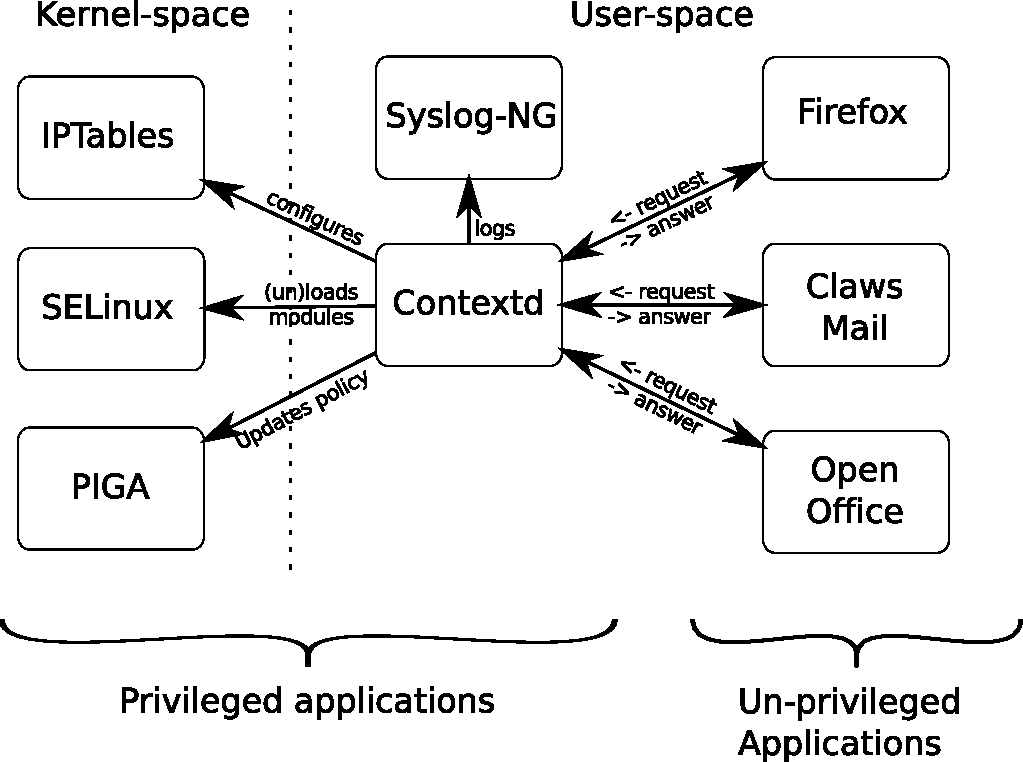
\includegraphics[scale=0.5]{architecture.pdf}
				\caption{The global architecture}
				\label{architecture}
			\end{figure}

			When receiving a request, the daemon checks whether it should change the domain. If it is the case, it warns all its plugins to update the configuration of
			their respective security component. Finally, the daemon send a signal to the registered application, warning that the current domain has changed. 
			These applications should now check if their current context is compatible with the new domain. If it is not, the application should go to a trash context explaining
			why the content of the application has changed.

\section{Experimentation}

This section presents the implementation of a secure desktop for Internet users.
This Operating System is part of the Security Challenge (SEC\&SI) funded by the French Research Agency (ANR).
The goal is to provide a secure system that allows a user to surf, to read/send mail, to make purchase and to pay his taxes on the Internet.

	\subsection{Secure desktop for Internet users}

This Operating System is based on GNU/Linux and provides a desktop interface with 2 kind of applications : a web browser (mozilla firefox) and an email client (clawsmail).
	
			\begin{figure*}[ht!]
				\centering
				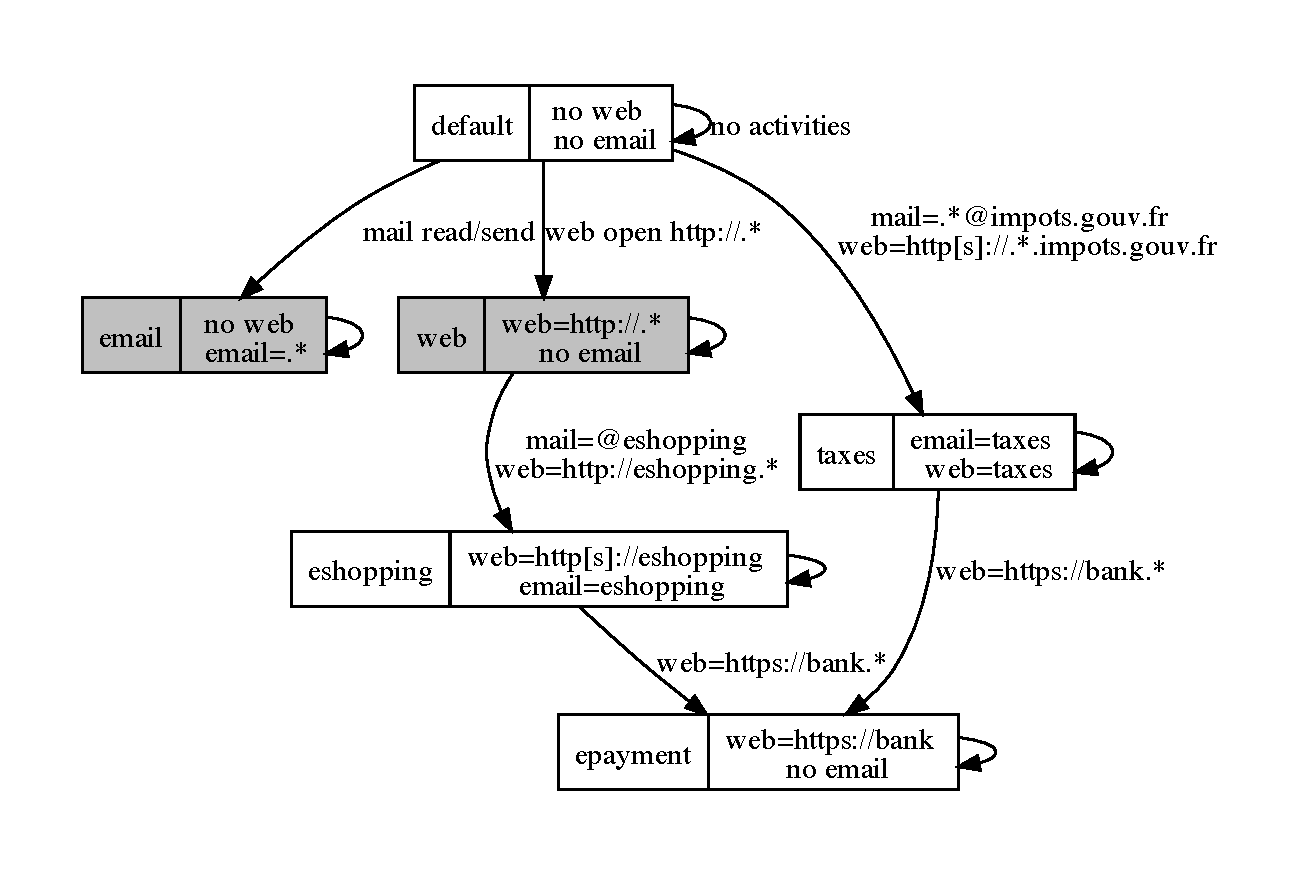
\includegraphics[scale=0.8]{transitions.pdf}
				\caption{Domains and Domain transition rules}
				\label{transitions}
			\end{figure*}

		\subsubsection{Domain}

The figure \ref{transitions} represents the domains and the domain transition rules.
Each node corresponds to a domain (domain name on left part) and it describes the activities allowed in this domain (right part).
Each arrow corresponds to a domain transition and it indicates the condition of the transition.
The domain filled in gray color are considered as untrusted domains, the other domains are used in order to confine the user when he want to buy something or he want to pay his taxes.
This implementation considers 6 domains :
\begin{itemize}
\item \textbf{Default} : when the system boot, the user enters to the default domain waiting for an activity that requires a transition.
The user can do nothing in this domain, he has no access to the Web and he cannot read/send emails.
\item \textbf{Email} : this domain allows the user to read/send email. He can access to all emails excepting emails from other contexts. 
This domain is considered as untrusted and the user can use it in order to consult or send personal or not confidential emails.
For example, he cannot read emails coming from  taxes services or eshopping sites.
\item \textbf{Web} : this domain allows the user to navigate on the Web. 
This domain is considered as untrusted and the user can use it in order to navigate on the Web.
He can consult each page that begins with \texttt{http://} excepting URLs that match other domains.
\item \textbf{Taxes} : if the user enters an URL that match \texttt{http[s]://.*.impots.gouv.fr}, he enters in the trusted domain that allows it to declare his taxes. He have access to his personal certificate used for the authentication on the taxes site.
When he has finish his declaration, he is redirected on his bank site, in order to pay his taxes, and the system transits to the Epaiment domain.
\item  \textbf{Eshopping} : this domain allows the user to navigate on eshopping site and secure signed site.
He can consult a white list of eshopping site and buy something on the Web.
This domain is considered has trusted and when the user want to pay his purchase, he transits to the Epayment domain.
\item \textbf{Epayment} :
this domain is the only one authorized to consult secure bank sites in order to confirm a payment.
\end{itemize}

		\subsubsection{Domain Transitions}

The domain transition rules are entry-point of a new domain. 
In the figure~\ref{transitions}, the user can only enter in a new domain that is more sensible that the preceding.
When a transition occurs, each application is reconfigured in order to lose information about the preceding.
For example, the firefox cache, history and copy/cut cache are cleaned.
In the case of the application environment cannot be cleaned, the contextd daemon can stop and then restart the application in the new domain.

If a user, in domain $A$, performs an activity that match the rules of a domain $B$ :
\begin{itemize}
\item If a transition between $A$ and $B$ exists, he can transit to the domain $B$;
\item If he refuses the transition, the request is denied and a error page is showed;
\item If no transition exist, the request is denied and a error page is showed;
\end{itemize}

If the user want to return to the default domain, he must close is session. It is actually the only solution that cleans up totally the user process environment (Xorg server).

The figure~\ref{transitions} represents the following transitions :
\begin{itemize}
\item \textbf{default to email} : the user opens clawsmail and he reads or sends a not confidential email;
\item \textbf{default to web} : the user opens firefox and he enters an untrusted URL;
\item \textbf{default to taxes} : the user enters an URL or read/send an email relative to the taxes web site;
\item \textbf{web to eshopping} : the user enters an URL or read/send an email relative to an eshopping web site (in the white list);
\item \textbf{eshopping to epayment} : the user is redirected to a secure bank site;
\item \textbf{taxes to epayement} : the user is redirected to a secure bank site;
\end{itemize}

			
	\subsection{Security Mechanism Details}
	
		\subsubsection{Applications control}

\paragraph{Web Browser}
An extension is installed in the web browser in order to intercept the URL entered by the user.
The contextd daemon controls this URL and decides if this URL is valid, allowed or required a transition.
If the URL is denied or the user refuses the transition, an error page is showed.
When a domain transition occurs, all open tab, that not respect the new domain rules, are closed.

\paragraph{Email client}
An other extension is installed in the email client in order to control the read and the send of email.
When the user wants to read a message, he can open it only if the mail header (\textit{from}, \textit{to}, ...) match the rules of the current domain and does not match the rules of other domain.
In order to control the send or the forward of email, the user can only send mail from the mail readable from the current domain to sender allowed in this domain.
When a domain transition occurs, all popup (send or forward message popup) are closed and the current message could be hidden if this message does not respect the current rules.

For example, in the Mail domain, an user can read his personal mail and forward it to an other user excepting taxes or eshopping contacts.
In the Taxes domain, he can only read/send/forward mail from/to taxes services.

	
		\subsubsection{Mandatory Access Control}

\paragraph{Firewall}
The firewall controls dynamically the flows between the user environment and the Internet.
When the user opens an URL and if this URL is allowed, the contextd daemon allows the IPs of the web site in the firewall.
If the user open a new URL or a domain transition occurs, the last set of IPs is removed from the firewall and the news are allowed.

When the user opens the mail client, the connection between the mail client and the mail server is opening during the recovering of the emails. If the user sends a mail, the connection is opening during the send.

Moreover, the firewall is used with SELinux packet marking capabilities in order to control flow between the applications and the Internet.
For example, firefox is the only application allowed opening a connection on the port http and https (80 and 443), only the mail client can connect to a mail server on the imaps/pops ports.

\paragraph{SELinux}

Contextd allows loading dynamically SELinux modules in order to modify the mandatory access control rules.
This capability allows changing the access control rules and the rights of applications.
For each domain, contextd load two new SELinux modules for clawsmail and firefox.
Each module restricts the privileges of these applications.
For example, in the Web and Mail domains, these applications cannot read files containing sensible data like files containing private keys or files in the home directory.
When the user is in the Taxes domain, firefox is able to read the file containing the user certificate in order to perform the authentication.
Moreover, when the user is able to create a file in a domain (save a mail, save a web page), this file is labeled with a identifier of this domain. 
When the user transits to an other domain, he is not able to read this file.
So, file saved in the Taxes domain are only readable in this domain.

\paragraph{PIGA}

As described in~\cite{SHPCS09}, current access control mechanism can only control direct interactions.
For example, SELinux can only control that an user cannot read a file.
But indirect access, like information flow cannot be controlled.
For example, an user reads information from a file and sends it to a user that cannot directly read it.
PIGA allows controlling this kind of activities.
Moreover, PIGA is based on the definition of security properties, written in the Security Property Language, and it prevents against the apparition of activities (directs or indirects) that violate these security properties.

The following security properties have been defined for this Operating System :
\begin{itemize}
\item an user cannot violate the integrity of the applications;
\item an user cannot violate the integrity of the system files;
\item an application cannot read its configuration after its execution. This property prevents against the divulgation of information (as login or password) contained in the configuration files of firefox and clawsmail;
\item an user cannot write and then execute a file. This property prevents against the download followed by the execution of a file.  
\item an user cannot write a file and then execute it with an interpreter. This property prevents against the download followed by the execution of a script.
\item an user can only execute a set of trusted application. This property is an implementation of a Trusted Path Execution (TPE).
\item each application has is proper TPE in order to specify its specific dependancies (libraries, ...);
\item an user can only access indirectly (information flow) to data that he can access directly. For example, if a user access to a more privileged account by using \textit{su} or \textit{sudo}, he cannot access to more information.
\end{itemize}

Moreover some properties are dynamically changed in order to apply supplementary confinement depending of the domain.
For example, in the untrusted domains, the user cannot violated the confidentiality of trusted files like files containing certificates, secret keys or sensitive data.

\section{Conclusion}
Our end-to-end security approach has been successfully integrated within an lightweight Linux Desktop, called PIGA-OS, in the context of the Security Challenge (SEC\&SI)  funded by the French Research National Agency (ANR). Currently, PIGA-OS wined the first round of that challenge. The other approaches deal with Virtualizated Systems. That challenge shows that the cooperation between the different protection
mechanisms provides even a more advanced protection than multiple
virtualized systems that are coordinated together. 


\bibliographystyle{plain}
\bibliography{biblio}

\end{document}
